\documentclass[8pt]{beamer}

\setbeamertemplate{background canvas}[vertical shading][bottom=cyan!10,top=blue!10]

\usetheme{Warsaw}
\usefonttheme[onlysmall]{structurebold}

% pour le fichiers .pdf
\usepackage{graphicx}
\usepackage{color}
% pour les fichiers .png
% \usepackage{pgf,pgfarrows}
% \usepackage{pgf,pgfarrows}
\usepackage{amsmath,amssymb}
\usepackage{textcomp}
\usepackage{Math_Notations}
\usepackage{multitoc}
\usepackage{mdwtab}
\setbeamercovered{dynamic}
\DeclareMathOperator*{\argmin}{argmin}

\title[OpenTURNS Developer training]{OpenTURNS Developer training: first steps}
\author[OpenTURNS Consortium, 2019]
{
  Trainer : Sofiane Haddad \\
  Airbus \\
  sofiane.haddad@airbus.com
}



\date[May 14-17th 2019]
{
  Developers training \\

  \begin{center}
    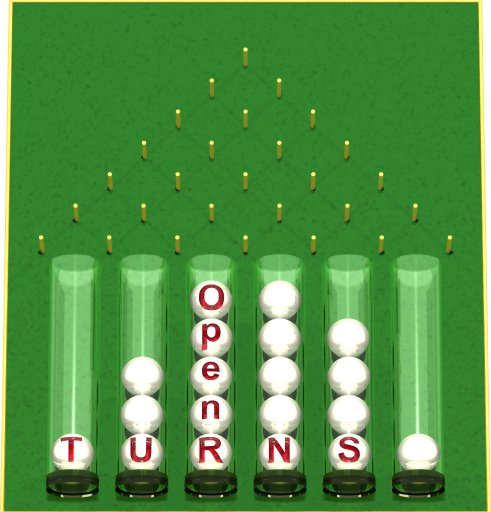
\includegraphics[height=2cm]{logoOT.jpg}
  \end{center}
}

\subject{OpenTURNS Developers Training}

\begin{document}

\frame{\titlepage}

% necessaire pour la table des matieres
\part{Main part}

% table des matieres
\begin{frame}
  \frametitle{OpenTURNS: first steps}
  \tableofcontents[part=1]
\end{frame}

\section{Navigation in the source code}

%%%%%%%%%%%%%%%%%%%%%%%%%%%%%%%%%
% Navigation in the source code %
%%%%%%%%%%%%%%%%%%%%%%%%%%%%%%%%%
\begin{frame}
  \frametitle{Navigation in the source code}
  \begin{block}{The Uniform distribution}
    \begin{itemize}
      \item Locate the class within the library source code;
      \item Follow its inheritance graph in order to explore the Bridge pattern;
      \item Locate the associated regression test;
      \item Execute the test;
      \item Locate its SWIG interface file and its associated Python module;
      \item Execute the associated python test.
    \end{itemize}
  \end{block}
\end{frame}


\section{Library development}

%%%%%%%%%%%%%%%%%% 
% Global picture %
%%%%%%%%%%%%%%%%%% 
\begin{frame}
  \frametitle{Library development 1/2}
  \begin{block}{Projects}
    \begin{enumerate}
      \item Weighted interpolation: create a new NumericalMathEvaluation that interpolate between points of a NumericalSample using weighted kernel interpolation.
        \begin{equation}
          f(\vect{x})=\alpha\sum_{i=0}^{N-1}K(\vect{x}-\vect{X}^i)\vect{Y}^i
        \end{equation}
where $K$ is a given Distribution and $\alpha$ is a normalization factor.
      \item CloudMesher: mesh generation over a cloud of points using kernel mixture, pca, rotation, then levelset mesher on an interval
      \item ClenshawCurtis 1-d integration: https://people.maths.ox.ac.uk/trefethen/cctalk.pdf + ClenshawCurtisProductExperiment
      \item TawnCopula/JoeCopula/MaxCopula 2-d copulas
    \end{enumerate}
  \end{block}
\end{frame}

\begin{frame}
  \frametitle{Library development 2/2}
  \begin{block}{Projects}
    \begin{enumerate}
      \setcounter{enumi}{4}
      \item Extend archimedian copulas from 2-d to $n$-d (FarlieGumbelMorgenstern, FrankCopula, ClaytonCopula, AliMikhailHaqCopula)
      \item ArchiMaxCopula, see ExtremeValueCopula
      \item Extend ComposedDistribution to accept a list of n-d distributions
      \item Add a method to SobolSimulationAlgorithm to draw sobol indices (openturns/issues/1001)
    \end{enumerate}
  \end{block}
\end{frame}



\section{Module development}

\begin{frame}
  \frametitle{Module development}
  \begin{block}{Projects}
    \begin{enumerate}
      \item Convert the IntegralCompoundPoisson distribution python module into an OpenTURNS C++ module
      \item Create a RandomVector distributed uniformly over an $n$ dimensional sphere/ball/simplex;
    \end{enumerate}
  \end{block}
\end{frame}
\end{document}

